\documentclass[
10pt, % Main document font size
a4paper, % Paper type, use 'letterpaper' for US Letter paper
oneside, % One page layout (no page indentation)
%twoside, % Two page layout (page indentation for binding and different headers)
headinclude,footinclude, % Extra spacing for the header and footer
BCOR=5mm, % Binding correction
table,
]{scrartcl}

%%%%%%%%%%%%%%%%%%%%%%%%%%%%%%%%%%%%%%%%%
% Arsclassica Article
% Structure Specification File
%
% This file has been downloaded from:
% http://www.LaTeXTemplates.com
%
% Original author:
% Lorenzo Pantieri (http://www.lorenzopantieri.net) with extensive modifications by:
% Vel (vel@latextemplates.com)
%
% License:
% CC BY-NC-SA 3.0 (http://creativecommons.org/licenses/by-nc-sa/3.0/)
%
%%%%%%%%%%%%%%%%%%%%%%%%%%%%%%%%%%%%%%%%%

%----------------------------------------------------------------------------------------
%	REQUIRED PACKAGES
%----------------------------------------------------------------------------------------

\usepackage[
nochapters, % Turn off chapters since this is an article        
beramono, % Use the Bera Mono font for monospaced text (\texttt)
eulermath,% Use the Euler font for mathematics
pdfspacing, % Makes use of pdftex’ letter spacing capabilities via the microtype package
dottedtoc % Dotted lines leading to the page numbers in the table of contents
]{classicthesis} % The layout is based on the Classic Thesis style

\usepackage[margin=1.4in]{geometry}

\usepackage[T1]{fontenc} % Use 8-bit encoding that has 256 glyphs

\usepackage[utf8]{inputenc} % Required for including letters with accents

\usepackage{graphicx} % Required for including images
\graphicspath{{Figures/}} % Set the default folder for images

\usepackage{enumitem} % Required for manipulating the whitespace between and within lists

\usepackage{lipsum} % Used for inserting dummy 'Lorem ipsum' text into the template

\usepackage{subfig} % Required for creating figures with multiple parts (subfigures)

\usepackage{amsmath,amssymb,amsthm} % For including math equations, theorems, symbols, etc

\usepackage{varioref} % More descriptive referencing

\usepackage{tabularx}

\usepackage{changepage}

\usepackage{pdfpages}

\usepackage[toc,page]{appendix}

\usepackage{float}

%\usepackage[table,xcdraw]{xcolor}

\usepackage{array,multirow}

\usepackage{booktabs}

%----------------------------------------------------------------------------------------
%	THEOREM STYLES
%---------------------------------------------------------------------------------------

\theoremstyle{definition} % Define theorem styles here based on the definition style (used for definitions and examples)
\newtheorem{definition}{Definition}

\theoremstyle{plain} % Define theorem styles here based on the plain style (used for theorems, lemmas, propositions)
\newtheorem{theorem}{Theorem}

\theoremstyle{remark} % Define theorem styles here based on the remark style (used for remarks and notes)

%----------------------------------------------------------------------------------------
%	HYPERLINKS
%---------------------------------------------------------------------------------------

\hypersetup{
%draft, % Uncomment to remove all links (useful for printing in black and white)
colorlinks=true, breaklinks=true, bookmarks=true,bookmarksnumbered,
urlcolor=webbrown, linkcolor=RoyalBlue, citecolor=webgreen, % Link colors
pdftitle={}, % PDF title
pdfauthor={\textcopyright}, % PDF Author
pdfsubject={}, % PDF Subject
pdfkeywords={}, % PDF Keywords
pdfcreator={pdfLaTeX}, % PDF Creator
pdfproducer={LaTeX with hyperref and ClassicThesis} % PDF producer
} % Include the structure.tex file which specified the document structure and layout

\hyphenation{Fortran hy-phen-ation} % Specify custom hyphenation points in words with dashes where you would like hyphenation to occur, or alternatively, don't put any dashes in a word to stop hyphenation altogether

%----------------------------------------------------------------------------------------
%	TITLE AND AUTHOR(S)
%----------------------------------------------------------------------------------------

\title{\normalfont\spacedallcaps{\textbf{FSE Development Board}} \\[2ex] \LARGE\spacedallcaps{Reference Manual}} % The article title
\author{\spacedlowsmallcaps{Frederic Afadjigla}} 
%\date{\small{(\today)}} 
\date{\small{Decembre 22, 2018}} 
%----------------------------------------------------------------------------------------


\begin{document}
%----------------------------------------------------------------------------------------
%	HEADERS
%----------------------------------------------------------------------------------------

\renewcommand{\sectionmark}[1]{\markright{\spacedlowsmallcaps{#1}}} % The header for all pages (oneside) or for even pages (twoside)
%\renewcommand{\subsectionmark}[1]{\markright{\thesubsection~#1}} % Uncomment when using the twoside option - this modifies the header on odd pages
\lehead{\mbox{\llap{\small\thepage\kern1em\color{halfgray} \vline}\color{halfgray}\hspace{0.5em}\rightmark\hfil}} % The header style
\pagestyle{scrheadings} % Enable the headers specified in this block

%----------------------------------------------------------------------------------------
%	TITLE
%----------------------------------------------------------------------------------------
\makeatletter
\def\@maketitle {

	%
\includegraphics[width = 40mm]{logoBW}\\[8ex]
	\begin{center}
		{\huge \bfseries \sffamily \@title }\\[4ex] 
		{\Large  \@author}\\[1ex] 
		\@date\\[8ex]
		
\includegraphics[width = 40mm]{logoBW} \\[20ex] 
		\end{center}
}
\makeatother
\thispagestyle{empty}

\maketitle % Print the title/author/date block

%----------------------------------------------------------------------------------------
%	TABLE OF CONTENTS & LISTS OF FIGURES AND TABLES
%----------------------------------------------------------------------------------------
\setcounter{tocdepth}{2} % Set the depth of the table of contents to show sections and subsections only

\tableofcontents % Print the table of contents
\listoffigures % Print the list of figures
\listoftables % Print the list of tables

%----------------------------------------------------------------------------------------
%	ABSTRACT
%----------------------------------------------------------------------------------------
\section*{Abstract} % This section will not appear in the table of contents due to the star (\section*)
The purpose of this document is to give the reader an overview about the FSEDevBoard's hardware. This plattform will be use during FSE workshops. Principal hardware components of the board and interfaces will be briefly described.

%
\newpage
%

%----------------------------------------------------------------------------------------
%	INTRODUCTION
%----------------------------------------------------------------------------------------
\section{Introduction}
This breakout board was build with the intention to add some additional features to the Raspberry Pi such as 8 Analog Digital Converter Pins, 2 DC Brushed Motor driver interfaces with TB6612FNG, 8 bidirectional level converted IOs (5V <-> 3.3V), 16-channel 12-bit PWM with PCA9685, one RGB LED and one Pushbutton. The following chapter will bring some light in how to interact with those functionalities.

%----------------------------------------------------------------------------------------
%	FSEDevBoard's Components
%----------------------------------------------------------------------------------------
\section{FSEDevBoard and its Components}
Top and bottom view of the board are shown in figure ~\vref{fig:Top view of board} and figure ~\vref{fig:Bottom view of board}. Brief Overview of the board can be taken from figure ~\vref{fig:FSEDevBoard_overview}. All Jumpers are placed on the top to ease connection with jumper wires.
Powering the board and the Pi can done via the micro USB port of the Raspberry Pi or via the Jumper \textbf{J2}. Please make sure \textcolor{red}{not to connect both at the same time} or this will destroy both boards. A battery voltage of maximum 15V can be connected to that jumper. This voltage will be used to drive both DC Motors and will be break down to 5V via a linear voltage regulator and provided to the Raspberry Pi.

\begin{figure}[h]
\minipage{0.48\textwidth}
  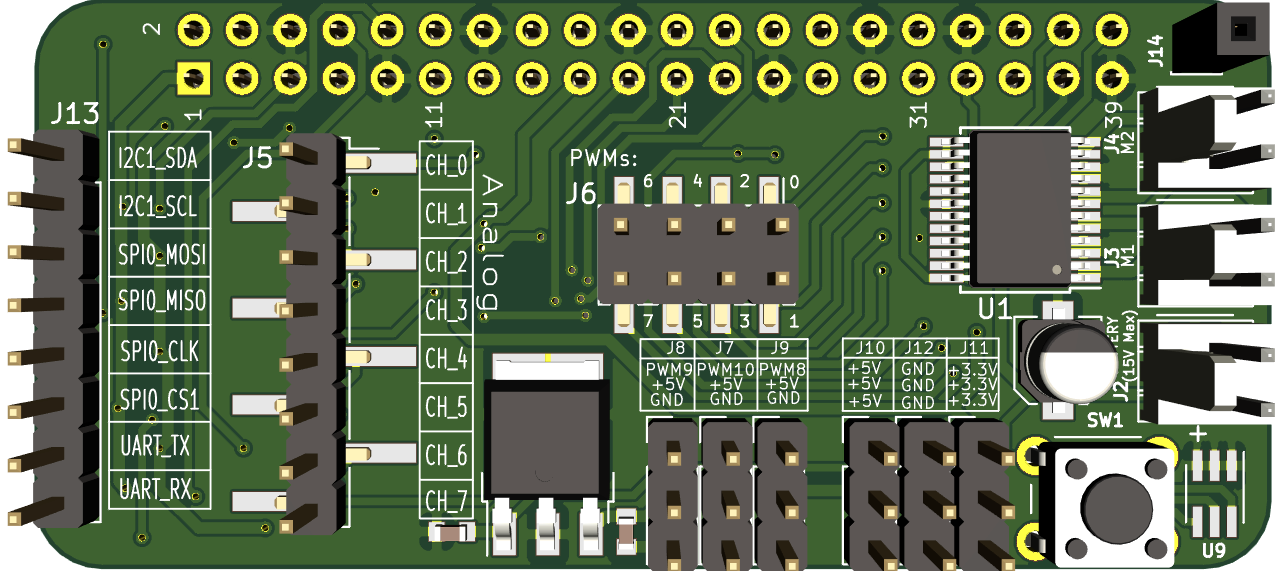
\includegraphics[width=\linewidth]{topView}
  \caption{Top view of board}\label{fig:Top view of board}
\endminipage\hfill
\minipage{0.48\textwidth}
  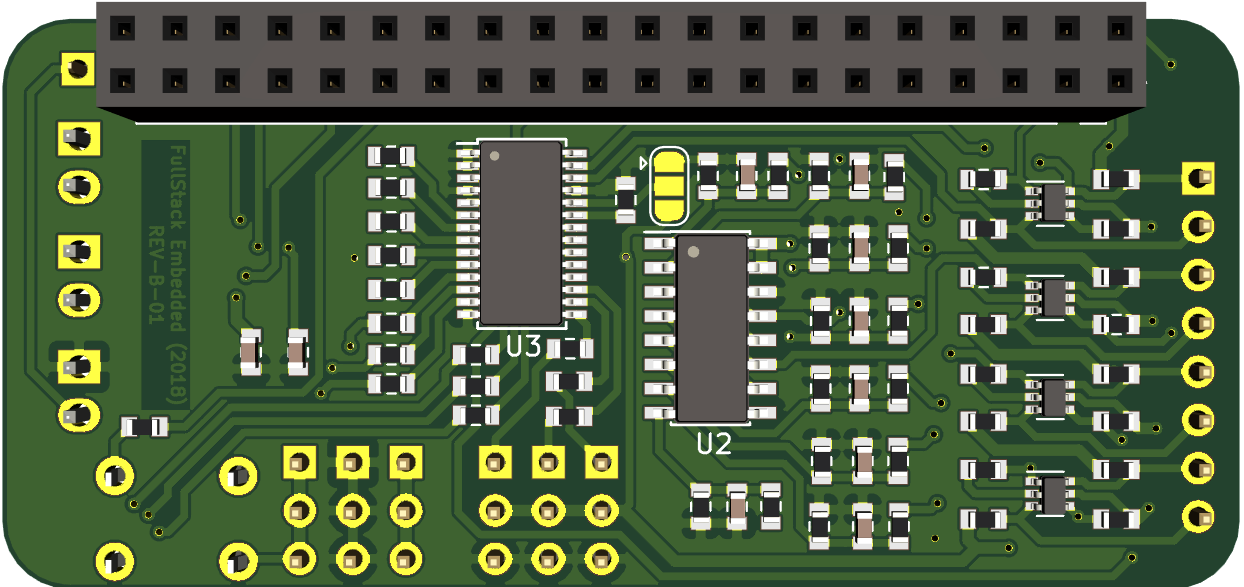
\includegraphics[width=\linewidth]{bottomView}
  \caption{Bottom view of board}\label{fig:Bottom view of board}
\endminipage
\end{figure}

\begin{figure}[h]
\centering
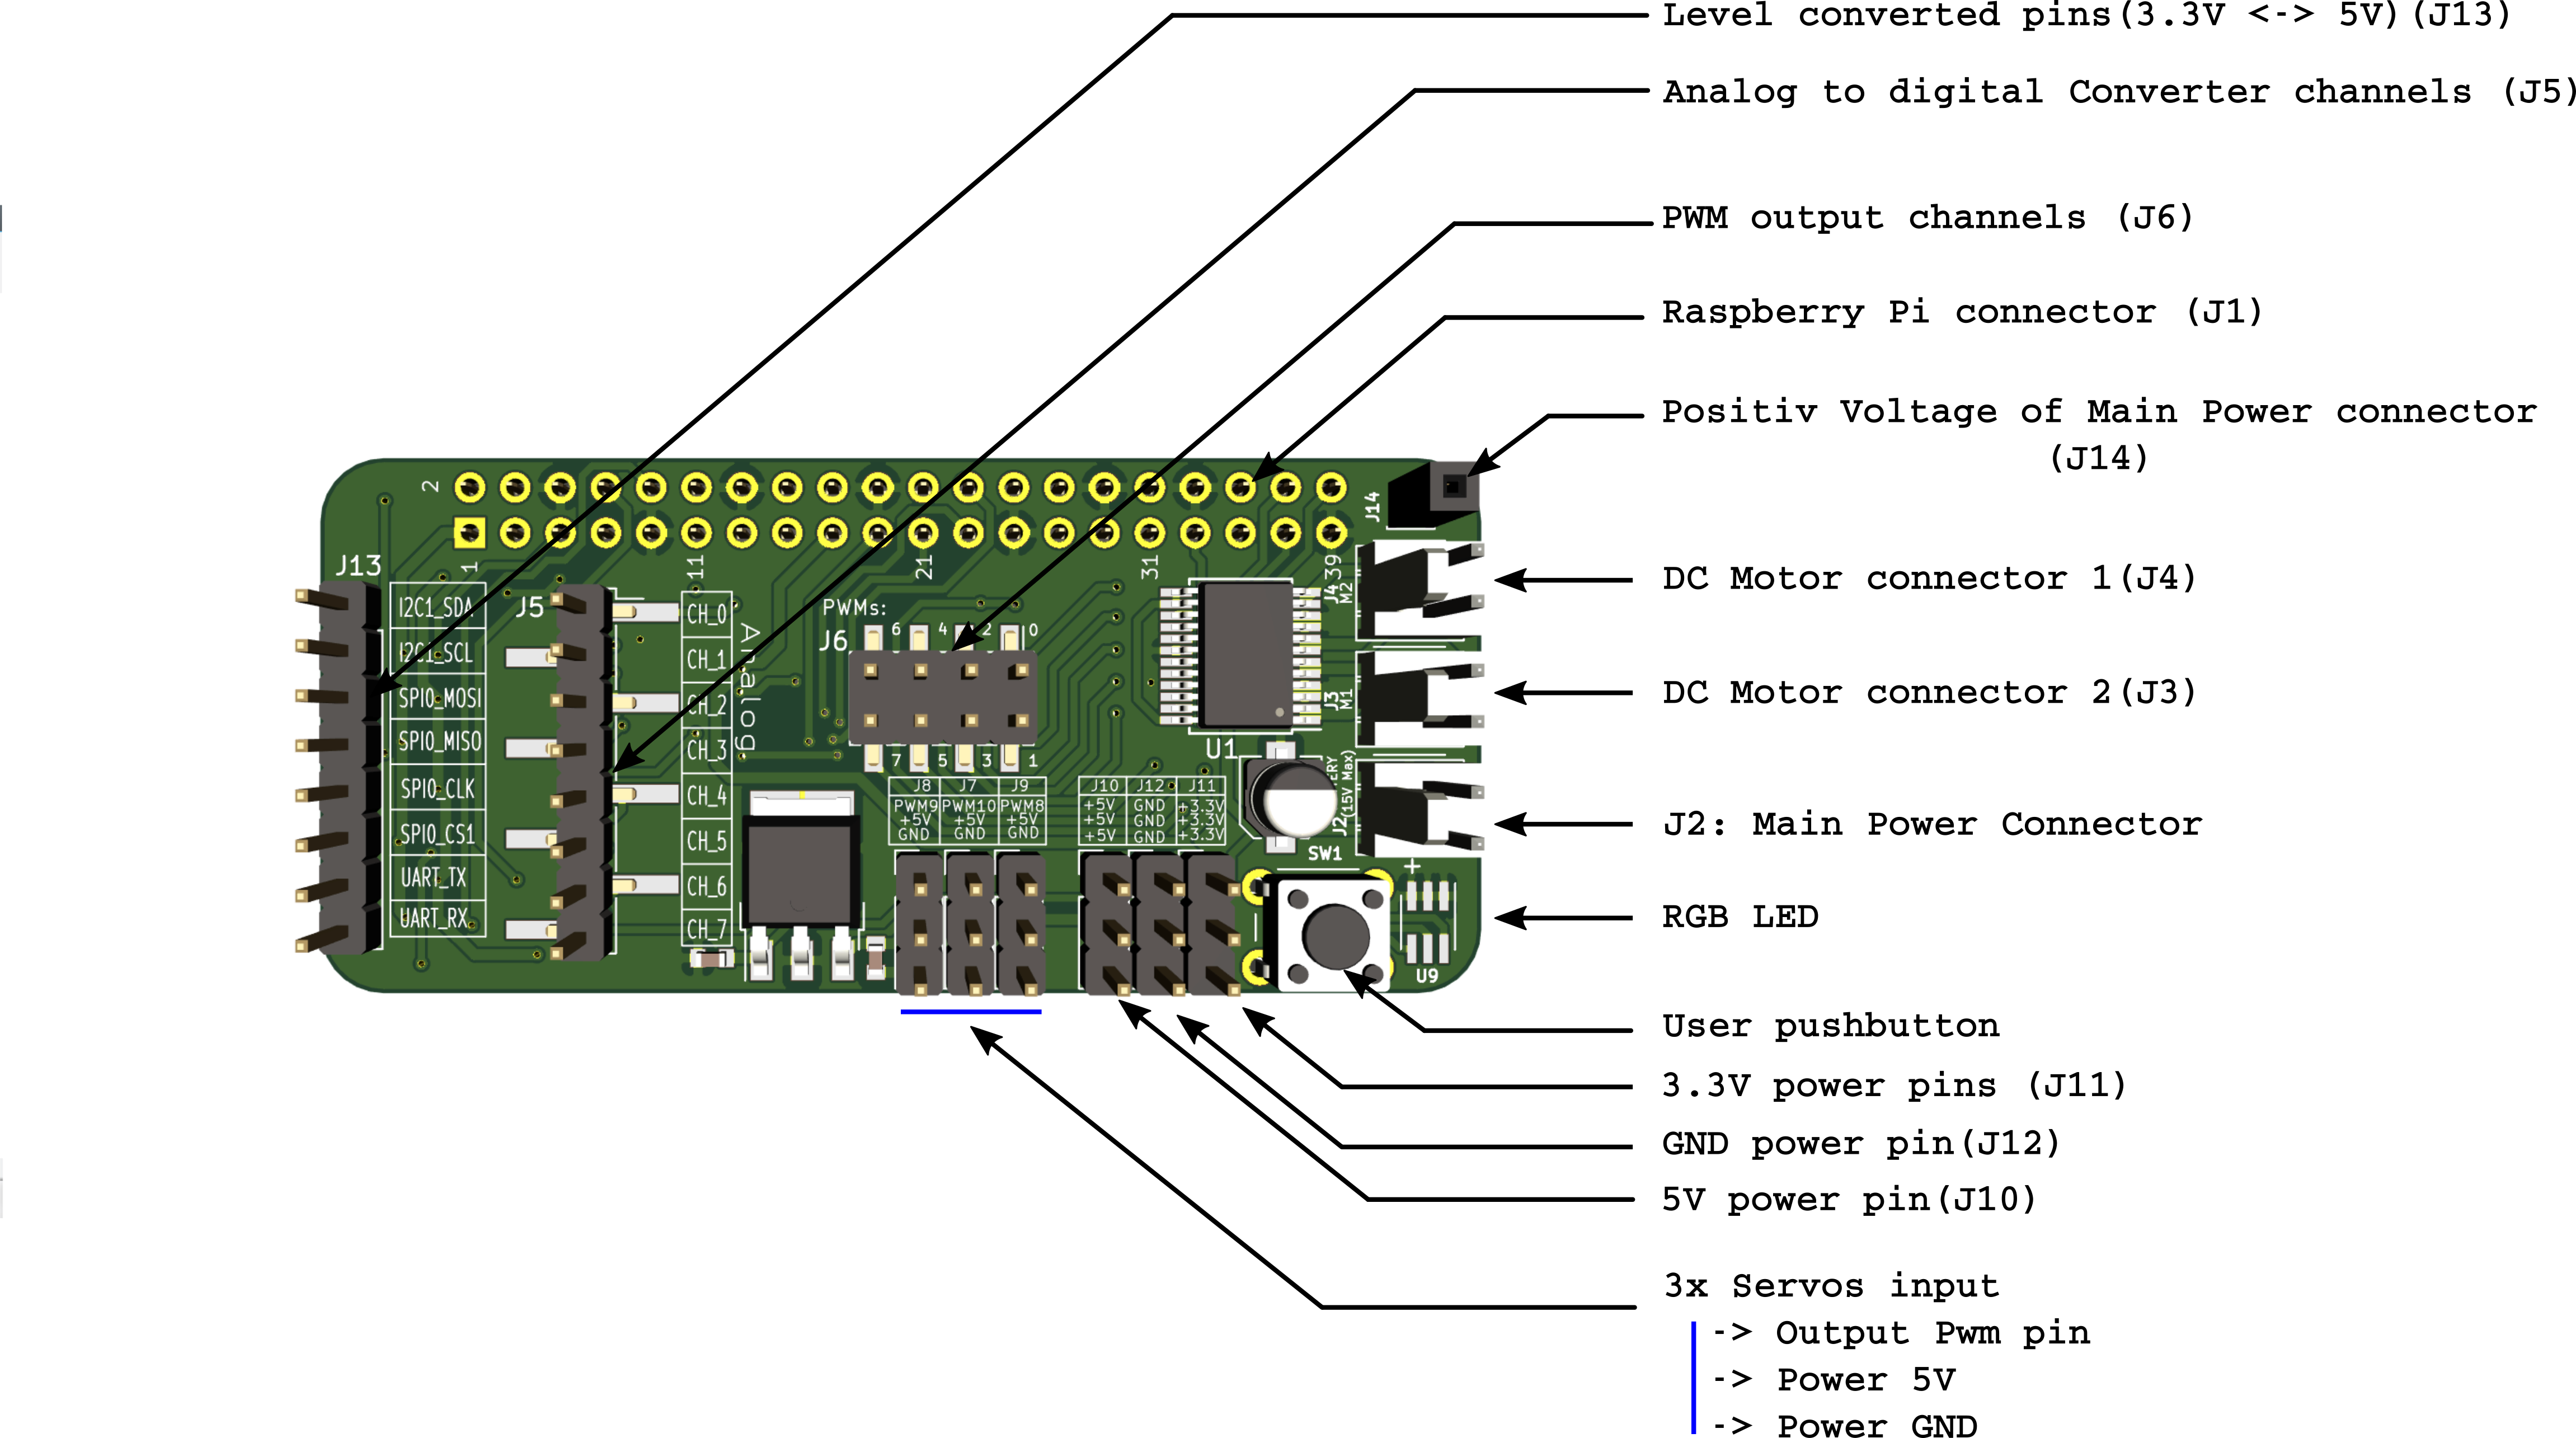
\includegraphics[width=1\columnwidth]{FSEDevBoard_overview}
\caption[FSEDevBoard Overview]{FSEDevBoard Overview}
\label{fig:FSEDevBoard_overview}
\end{figure}

\subsection{Analog Inputs for Raspberry Pi Using the MCP3008}
The MCP3008 is a low cost 8-channel 10-bit analog to digital converter. The MCP3008 connects to the Raspberry Pi using a serial peripheral interface (SPI) serial connection. 

\begin{figure}[h]
\centering
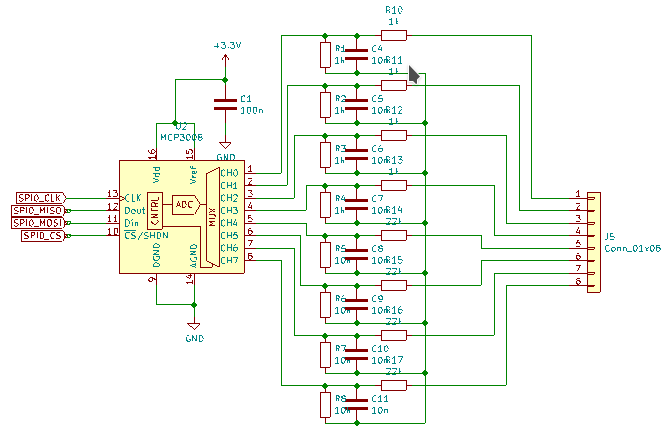
\includegraphics[width=1\columnwidth]{MCP3008} 
\caption[MCP3008 schematic]{MCP3008 schematic}
\label{fig:MCP3008}
\end{figure}

\begin{table}[H]
\centering
\begin{tabular}{lr}
\hline
\textbf{SPI Pins} & \textbf{Raspberry Pi pin} \\
\hline
SCLK (Serial Clock)        & GPIO11 \\
MOSI (Master Out Slave In) & GPIO10 \\
MISO (Master In Slave Out) & GPIO09 \\
CS   (Chip Select)         & GPIO25 \\
\hline
\end{tabular}
\label{tab:label}
\caption{MCP3008 SPI connection}
\end{table}

Voltage that are allowed to be connected to the MCP3008 have to be selected so that \(V_{out}\) muss be less than 3.3V(\(V_{ref}\)). \(V_{out}\) is the voltage that can be measured after the voltage dividers. All 4 first channels (0,1,2 and 3) are designed to have a measuring range of 0-5V DC. The last 4 Channels can measure up to 10V.
\(V_{out[0-3]}\) for channels 0,1,2 and 3 can be calculated as:

\[ V_{ out[0-3] } = \frac{ R_{6} }{ R_{5} + R_{6} } * V_{in}  = 0.5* V_{in}\]

In case of channel 4,5,6 and 7:

\[ V_{out[4-7]} = 0.316 * V_{in}\]

Jumper J14 can be connected to one of Channel 4 to 7 to measure the batterie voltage of the Board.

\subsection{Level Converted Pins}
Precautions have to be taken when connecting 5V devices to the raspberry pi since the Pi is \textbf{not 5V tolerant}. The user has to make sure that voltage going to the Raspberry Pi do not exceed 5V. There are many ways to handle the matter. Easiest way is probably using voltage dividers with 2 resistors. Care has to be taken to the direction of the voltage since those are not bidirectional. More robust way which gives you biderctional capacity is by using an Integrated circuit (IC) or using the circuitry like I did in figure  ~\vref{fig:LevelConverter} based on one N-Channel Mosfet.


\begin{figure}[h]
\centering
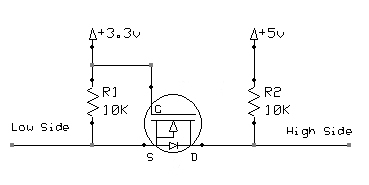
\includegraphics[width=0.7\columnwidth]{mosfet_level_converter} 
\caption[Level Converter]{Level Converter \footnotemark}
\label{fig:LevelConverter}
\end{figure}
\footnotetext{\label{levelConv}\url{http://www.hobbytronics.co.uk/mosfet-voltage-level-converter}}

\textbf{Low Side Control:} When the low side (3.3V) device transmits a '1' (3.3V), the MOSFET is tied high (off), and the high side sees 5V through the R2 pull-up resistor. When the low side transmits a '0' (0V), the MOSFET source pin is grounded and the MOSFET is switched on and the high side is pulled down to 0V.\footnote{see footnote \footref{levelConv}}

\textbf{High Side Control:} When the high side transmits a '0' (0V) the MOSFET substrate diode conducts pulling the lowside down to approx 0.7V, this is also low enough to turn the MOSFET on, further pulling the low side down. When the high side transmits a '1' (5V) the MOSFET source pin is pulled up to 3.3V and the MOSFET is OFF.

Note This works with I2C and other open collector type gates \footnote{see footnote \footref{levelConv}}


\begin{table}[H]
\centering
\begin{tabular}{cc}
\hline
\textbf{Pins} & \textbf{RPi pin} \\
\hline
1  & GPIO02 \\
2  & GPIO03 \\
3  & GPIO10 \\
4  & GPIO09 \\
5  & GPIO011 \\
6  & GPIO07 \\
7  & GPIO14 \\
8  & GPIO15 \\
\hline
\end{tabular}
\label{tab:label}
\caption{Level Converted Pins}
\end{table}
\subsection {DC Motor driver - TB6612FNG}
The TB6612FNG motor driver can control up to two DC motors at a constant current of 1.2A (3.2A peak). Two input signals (IN1 and IN2) can be used to control the motor in one of four function modes - clockwise (CW), counter-clockwise (CCW), short-brake, and stop. The two motor outputs (A and B) can be separately controlled, the speed of each motor is controlled via a PWM input signal with a frequency up to 100kHz. The STBY pin should be pulled high to take the motor out of standby mode.

Logic supply voltage (VCC) can be in the range of 2.7-5.5VDC, while the motor supply (VM) is limited to a maximum voltage of 15VDC. The output current is rated up to 1.2A per channel (or up to 3.2A for a short, single pulse).\\

Features:
\begin{itemize}
\item[•] Power supply voltage: VM=15V max, VCC=2.7-5.5V
\item[•] Output current: Iout=1.2A(average) / 3.2A (peak)
\item[•] Standby control to save power
\item[•] CW/CCW/short brake/stop motor control modes
\item[•] Built-in thermal shutdown circuit and low voltage detecting circuit
\item[•] All pins of the TB6612FNG broken out to 0.1" spaced pins
\item[•] Filtering capacitors on both supply lines
\end{itemize}

\begin{figure}[H]
\centering
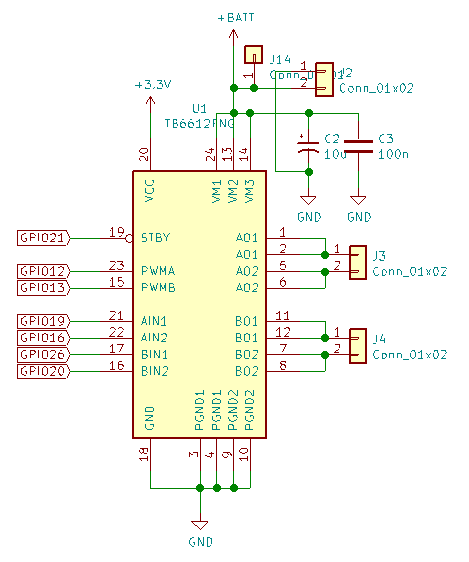
\includegraphics[width=0.65\columnwidth]{TB6612FNG} 
\caption[TB6612FNG schematic]{TB6612FNG schematic}
\label{fig:TB6612FNG}
\end{figure}
Let’s discuss the pinout for the TB6612FNG:


\newcolumntype{b}{X}
\newcolumntype{s}{>{\hsize=.3\hsize}X}
\newcolumntype{m}{>{\hsize=.5\hsize}X}

\begin{table}[H]
\centering
\begin{adjustwidth}{-1cm}{}
\resizebox{16cm}{!} {%
\begin{tabularx}{18cm}{smb}
\hline
\textbf{Pin Label} & \textbf{Function} & \textbf{Notes} \\
\hline
VM & Motor Voltage  & This is where you provide power for the motors (2.2V to 13.5V)\\
VCC & Logic Voltage & This is the voltage to power the chip and talk to the microcontroller (2.7V to 5.5V)\\
GND & Ground  & Common Ground for both motor voltage and logic voltage (all GND pins are connected)\\
STBY & Standby & Allows the H-bridges to work when high (has a pulldown resistor so it must actively pulled high)\\
AIN1/BIN1 & Input 1 for channels A/B   & One of the two inputs that determines the direction\\
AIN2/BIN2 & Input 2 for channels A/B   & One of the two inputs that determines the direction\\
PWMA/PWMB & PWM input for channels A/B & PWM input that controls the speed\\
A01/B01 & Output 1 for channels A/B  & One of the two outputs to connect the motor\\
A02/B02 & Output 2 for channels A/B  & One of the two outputs to connect the motor\\
\hline
\end{tabularx} } 
\end{adjustwidth}
\label{tab:label}
\caption{TB6612FNG connection}
\end{table}

When the outputs are set to High/Low your motor will run. When they are set to Low/High the motor will run in the opposite direction. In both cases, the speed is controlled by the PWM input.

\begin{table}[H]
\centering
\begin{tabular}{cccccc}
\hline
\textbf{In1}  & \textbf{In2} & \textbf{PWM} & \textbf{Out1} & \textbf{Out2} & \textbf{Mode} \\
\hline
H    & H   & H/L & L    &L     & Short brake\\
L    & H   & H   & L    & H    & CCW\\
L    & H   & L   & L    & L    & Short brake\\
H    & L   & H   & H    & L    & CW\\
H    & L   & L   & L    & L    & Short brake\\
L    & L   & H   & OFF  & OFF  & Stop\\
\hline
\end{tabular}
\caption{TB6612FNG Logic}
\label{tab:label}
\end{table}

%----------------------------------------------------------------------------------------
%	The Raspberry Pi pinout
%----------------------------------------------------------------------------------------
\section{The Raspberry Pi pinout}
The Raspberry Pi's GPIOs can be accessed over a standard male header on the board. Over the years the header expanded from 26 to 40 pins.There are 2 different numbering schemes you may encounter when referencing Pi pin numbers: (1) Broadcom chip-specific pin numbers and (2) P1 physical pin numbers. You’re usually free to use either number-system, but many programs require that you declare which scheme you’re using at the very beginning of your program. 
Green areas in Table \ref{table:Raspberry Pi Pinout} are representing free GPIOs which are not connected to anything on the FSEDevBoard. Therefore, you can safely add some new connections to those pins

\begin{table}[H]
\centering
\resizebox{\textwidth}{!}{%
\begin{tabular}{cccccc}
\hline
\textbf{FSEDevBoard}     & \textbf{Name}          & \multicolumn{2}{c}{\textbf{Pin Nbr}}                                      & \textbf{Name}          & \textbf{FSEDevBoard}     \\ \hline
                         & 3V3                    & \cellcolor[HTML]{C0C0C0}\textbf{1}  & \cellcolor[HTML]{C0C0C0}\textbf{2}  & 5V                     &                          \\
LV I2C1 SDA              & GPIO02 (SDA1, I2C)     & \cellcolor[HTML]{C0C0C0}\textbf{3}  & \cellcolor[HTML]{C0C0C0}\textbf{4}  & 5V                     &                          \\
LV I2C1 SCL              & GPIO03 (SCL1, I2C)     & \cellcolor[HTML]{C0C0C0}\textbf{5}  & \cellcolor[HTML]{C0C0C0}\textbf{6}  & GND                    &                          \\
\cellcolor[HTML]{32CB00} & GPIO04 (GPIO\_GCLK)    & \cellcolor[HTML]{C0C0C0}\textbf{7}  & \cellcolor[HTML]{C0C0C0}\textbf{8}  & GPIO14 (TXD0)          & LV UART TX               \\
                         & GND                    & \cellcolor[HTML]{C0C0C0}\textbf{9}  & \cellcolor[HTML]{C0C0C0}\textbf{10} & GPIO15 (RXD0)          & LV UART RX               \\
\cellcolor[HTML]{32CB00} & GPIO17 (GPIO\_GEN0)    & \cellcolor[HTML]{C0C0C0}\textbf{11} & \cellcolor[HTML]{C0C0C0}\textbf{12} & GPIO18 (GPIO\_GEN1)    & \cellcolor[HTML]{32CB00} \\
\cellcolor[HTML]{32CB00} & GPIO27 (GPIO\_GEN2)    & \cellcolor[HTML]{C0C0C0}\textbf{13} & \cellcolor[HTML]{C0C0C0}\textbf{14} & GND                    &                          \\
\cellcolor[HTML]{32CB00} & GPIO22 (GPIO\_GEN3)    & \cellcolor[HTML]{C0C0C0}\textbf{15} & \cellcolor[HTML]{C0C0C0}\textbf{16} & GPIO23 (GPIO\_GEN4)    & \cellcolor[HTML]{32CB00} \\
                         & 3V3                    & \cellcolor[HTML]{C0C0C0}\textbf{17} & \cellcolor[HTML]{C0C0C0}\textbf{18} & GPIO24 (GPIO\_GEN5)    & \cellcolor[HTML]{32CB00} \\
LV SPI0 MOSI             & GPIO10 (SPI\_MOSI)     & \cellcolor[HTML]{C0C0C0}\textbf{19} & \cellcolor[HTML]{C0C0C0}\textbf{20} & GND                    &                          \\
LV SPI0 MISO             & GPIO09 (SPI\_MISO)     & \cellcolor[HTML]{C0C0C0}\textbf{21} & \cellcolor[HTML]{C0C0C0}\textbf{22} & GPIO25 (GPIO\_GEN6)    & Push button              \\
LV SPI0 CLK              & GPIO11 (SPI\_CLK)      & \cellcolor[HTML]{C0C0C0}\textbf{23} & \cellcolor[HTML]{C0C0C0}\textbf{24} & GPIO08 (SPI\_CE0\_N)   & MCP3008 SPI0 CS          \\
                         & GND                    & \cellcolor[HTML]{C0C0C0}\textbf{25} & \cellcolor[HTML]{C0C0C0}\textbf{26} & GPIO07 (SPI\_CE1\_N)   & LV SPI0 CS1 (J13\_6)     \\
                         & ID\_SD (I2C ID EEPROM) & \cellcolor[HTML]{C0C0C0}\textbf{27} & \cellcolor[HTML]{C0C0C0}\textbf{28} & ID\_SC (I2C ID EEPROM) &                          \\
\cellcolor[HTML]{32CB00} & GPIO05                 & \cellcolor[HTML]{C0C0C0}\textbf{29} & \cellcolor[HTML]{C0C0C0}\textbf{30} & GND                    &                          \\
\cellcolor[HTML]{32CB00} & GPIO06                 & \cellcolor[HTML]{C0C0C0}\textbf{31} & \cellcolor[HTML]{C0C0C0}\textbf{32} & GPIO12                 & TB6612FNG PWMA           \\
TB6612FNG PWMB           & GPIO13                 & \cellcolor[HTML]{C0C0C0}\textbf{33} & \cellcolor[HTML]{C0C0C0}\textbf{34} & GND                    &                          \\
TB6612FNG AIN1           & GPIO19                 & \cellcolor[HTML]{C0C0C0}\textbf{35} & \cellcolor[HTML]{C0C0C0}\textbf{36} & GPIO16                 & TB6612FNG AIN2           \\
TB6612FNG BIN1           & GPIO26                 & \cellcolor[HTML]{C0C0C0}\textbf{37} & \cellcolor[HTML]{C0C0C0}\textbf{38} & GPIO20                 & TB6612FNG BIN2           \\
                         & GND                    & \cellcolor[HTML]{C0C0C0}\textbf{39} & \cellcolor[HTML]{C0C0C0}\textbf{40} & GPIO21                 & TB6612FNG STBY           \\ \hline
\end{tabular}%
}
\caption{Raspberry Pi Pinout}
\label{table:Raspberry Pi Pinout}
\end{table}


\begin{appendices}
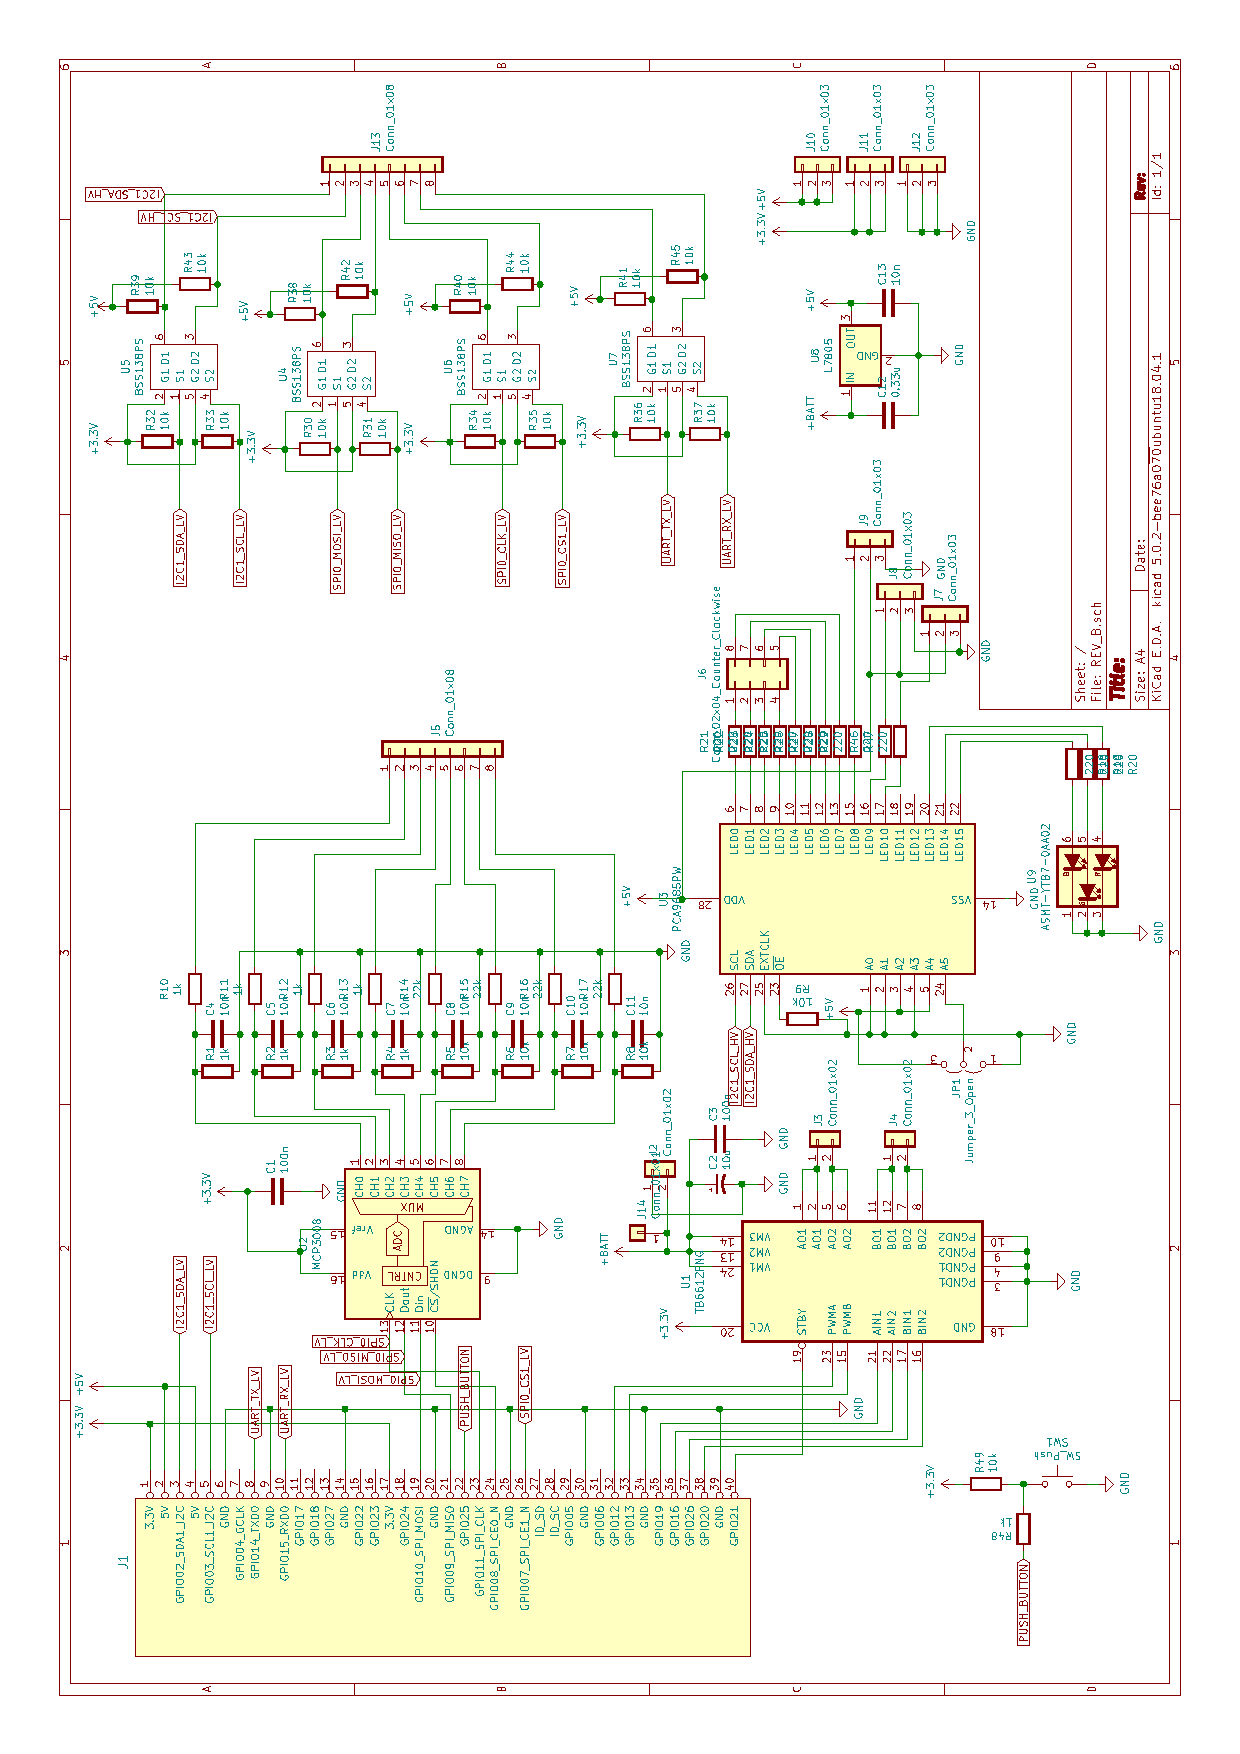
\includepdf[pages=-]{REV_B.pdf}
\end{appendices}




\end{document}

